\documentclass[9pt,technote]{IEEEtran}

\usepackage{hyperref,graphicx,cite}

\title{A Python-based Tobacco Classification Implementation}
\author{Chengxi Zhong\\ 
University of New South Wales\\ 
Student ID: z5301296\\
Email: t.zhong@student.unsw.edu.au
}

\begin{document}
\maketitle
\section{Introduction and Background}
\subsection{Introduction}
Tobacco is a plant that can be used for various purposes. Classification of tobacco against other plants can be distinguished using phenotypes. The phenotype of a plant describes its characteristics such as number of leaves, architecture, visual age or maturity level, height, leaf shape and so on.\cite{Phenotyp28:online} In this paper, we discuss a technique that can distinguish arabidopsis and tobacco, implemented using Python 3.6 and OpenCV\cite{OpenCV87:online} library.\\

The two plants have significantly different phenotypes. Arabidopsis have round, longer leaves while tobacco have sharp leaves. While human eyes can distinguish them easily, it is not the case for computers. Therefore, we are going to utilise algorithms that can distinguish the two types of leaves. In this paper, we discuss the implementation of techniques of supervised and unsupervised machine learning classification methods.\\

Since machine learning is needed, we should have a batch of images that are used to train a machine learning model with which the differentiation can be achieved. In this paper, we use the Plant Phenotyping Dataset as used in \cite{minervini2016finely} to train the classification model.
\begin{figure}[h!]
  \centering
  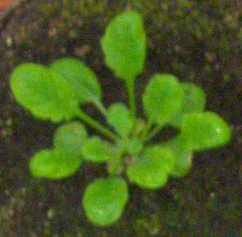
\includegraphics[width=0.25\textwidth]{ara2012_plant008_rgb}
  \caption{Example of Arabidopsis plant}
\end{figure}
\begin{figure}[h!]
  \centering
  \includegraphics[width=0.25\textwidth]{tobacco_plant034_rgb}
  \caption{Example of Tobacco plant}
\end{figure}
\subsection{Literature Review}
D.S.Guru et al. described a classification technique using \textit{K-nearest neighbour} (KNN) algorithm to classify flowers. \cite{guru2010texture} The author has used that method to classify different variants of flowers, which has inter-class variations and intra-class variations to be classified. This method is seriously considered due to the high similarities between the task mentioned in the paper prescribed and the task to be examined in this paper.


%---bibliography---%
\bibliography{Indiv_rep} 
\bibliographystyle{ieeetr}
\end{document}

